\documentclass[12pt,a4paper]{article}
\usepackage{amsfonts}
\usepackage{amsthm}
\usepackage{amsfonts}
\usepackage{amsmath}
\usepackage{amscd}
\usepackage{booktabs}
\usepackage[latin2]{inputenc}
\usepackage{t1enc}
\usepackage[mathscr]{eucal}
\usepackage{indentfirst}
\usepackage{graphicx}
\usepackage{hyperref}
\usepackage{graphics}
\numberwithin{equation}{section}
\usepackage{hyperref}
\usepackage[margin=2.9cm]{geometry}
\usepackage[outdir=./images/]{epstopdf}
\epstopdfsetup{outdir=./images/}
\usepackage{algorithm}
\usepackage{algpseudocode}

\algrenewcommand\algorithmicrequire{\textbf{Input:}}
\algrenewcommand\algorithmicensure{\textbf{Output:}}

\def\numset#1{{\\mathbb #1}}

\begin{document}
 
\title{Estimating Gaze Duration Error from Eye Tracking Data}

\author{
John Hawkins \\ email \href{mailto:john.hawkins@playgroundxyz.com}{john.hawkins@playgroundxyz.com} \\
} 

\maketitle

\section{Abstract}

Eye tracking technologies produce a series of timestamped gaze fixation points 
that can be attributed to objects within a subject's field of vision. 
These fixation points are often aggregated in order to generate a measurement
of the gaze duration in Area of Interest studies.
Error is typically measured on the basis of the variation between individual 
gaze fixation points and the intended point of fixation.
These underlying errors in fixation have no inherent transformation for making
a statement about error in gaze duration, even though they are expected to be
related.

In this work we develop an algorithm for estimating the error distribution of 
gaze duration measurement through Monte Carlo simulation using the content 
of an eye tracking calibration log file. 
We provide this algorithm in an open source application
to allow researchers to understand the error in their gaze duration measurements. 
We use this application to conduct experiments on the expected error bounds for 
different duration measurements across a fixed session length for a simulated 
area of interest study on a mobile device. 
The results indicate that error in gaze duration estimation is sensitive to
fixation error beyond a bound that will depend on the size of the area of interest 
and the comparative length of the viewing session.

\section{Introduction}

Eye tracking is an important technology with a wide variety of applications. 
It permits evaluation of software user interfaces\cite{Harezlak2015}, 
the development of new forms of software interaction, as well as a potential method of biometric identification\cite{Kasprowski2018}. Eye tracking has become a core tool for empirical 
investigations into human behaviour and is widely used as a method of measuring explicit 
attention to visual stimuli. 
It has been applied to study psychological phenomena ranging from cognition\cite{Brunye2019}
to mental health\cite{Duque2014,Rudich-Strassler2022}, and is now routinely used to evaluate 
advertising \cite{Hervet2011}. Eye tracking technology has allowed marketing researchers 
to study many factors that contribute to effective advertising, 
including brand recall \cite{Wedel2000},
the capture and tranfer of attention \cite{Pieters2004}, 
the impact of images of faces \cite{Djamasbi2010},
the attention effects of animation \cite{Hamborg2012},
and the relationship with social media posts \cite{Barreto2013}.

Increasingly, eye tracking applications are built using devices that employ 
machine learning models trained to predict fixation locations from a camera image.
While this approach to eye tracking may suffer in terms of accuracy, it can
open up possibilities for researchers in terms of reduced cost and increased scale
of experiments. As well as facilitating studies that head position restricting 
devices prevent\cite{Valtakari2021}.

The source of errors in eye tracking technology can be decomposed into a range of
independent sources that researchers need to consider\cite{Holmqvist2012}.
Unless they are properly addressed these sources of error can manifest themselves
as systematic biases across undesirable dimensions such as the age\cite{Dalrymple2018}
or ethnicity of subjects\cite{Blignaut2013}. Machine learning based eye tracking solutions
can be impacted by the variety of faces and lighting conditions in the training data. 
The errors in fixation point measurement for a given eye tracking solution are routinely
monitored and adjusted through a process called calibration, in which users are presented
a series or \emph{required fixation locations} (RFL) which are compared with measured 
points of fixation\cite{Hornof2002}. 
Improvements in the callibration process
are an ongoing focus for the development of algorithms\cite{Zhang2014,Hassoumi2019} 
and software tools\cite{ETCAL2018}. In some scenarios there are additional considerations
such as whether to use fixation data from individual eyes, or a composite 
signal\cite{Hooge2019}.

In eye tracking literature the error detected in the calibration process is classified
using two independent metrics; accuracy and precision. Accuracy is a measure for how
close, on average, the fixation points are to the true point of fixation.
Precision is the tendency for the measured locations to vary between subsequent measurements
for a given point of fixation\cite{Holmqvist2022}. This distinction
is critical because it forms the basis of methods that can correct for the kind of 
systematic bias observed with low precision eye tracking. It also been observed that
metrics of the precision in these models vary in the way they rank 
technologies\cite{Niehorster2020}. We can conclude from this that the patterns of 
systematic error in eye tracking
data are more complicated that can be quantifed by a single metric.

When fixation models are used sequentially for the purpose of estimating gaze duration
(as is commonly done in point of salience or advertising media studies), 
then there is the potential for the error
to either cancel out (reducing error in gaze duration estimation) or to compound
(increasing error in gaze duration). Which of these outcomes occurs will depend on the
specifics of the model and the conditions under which it is being used.
Influencing factors include the ratio of measured gaze duration to the 
total viewing time and the error profile of the gaze fixation technology.

The use of eye fixation models to estimate gaze duration (or dwell time) in Area of
Interest studies (AOI) was discussed by Holmqvist et al. \cite{Holmqvist2012}. The
authors simulated the impact of gaze fixation error by adding noise according to
manufacturer specifications to data sets of low margin areas of interest. We extend 
this idea to calculate probabilistic bounds on the error in gaze duration using
calibration data as a source of noise distribution that is specific to both the
study participants and the device/environment of the study. The result is an open
source application that may be used by a wide variety of reserachers to provide
error bounds on any gaze duration measurements.

\section{Methodology}

We estimate the gaze duration measurement error through a Monte Carlo simulation
using the eye tracking model's calibration file of fixation errors.
The error profile of the eye tracking model allows us to generate sequences of true
fixations and simulate measured fixations with the observed error of the model.
These sequences of true and measured fixation are then converted into a distribution
of expected gaze duration on a specifc area of interest, for a given measurement. 

The algorithm consists of two core steps, first estimating the distrubtion of measurements
for a given true duration. Secondly, inverting this into the distribution of true
gaze durations for a given measurement. Note, that the algorithm requires that the area of
interest be defined as a fixed bounding box and that the distributions are estimated for
a fixed session length. This session length is the total period of time that the area of
interest was in a subject's field of view, and thus represents the maximum possible gaze
duration.

\subsection{Measurement Distribution}

In the first stage of the methodology we provide an estimate of the distribution of measured
durations for all possible true gaze durations. These distributions are produced by generating
random fixation paths across the available screen dimensions, and adding noise that is 
drawn from the calibration data to make it consistent with the observed properties of the gaze model.
This produces a set of distributions that capture the expected
variation in measurement depending on the length of true fixation.

Formally stated this is the probability distribution over measured durations $\hat{d}$ given a
known duration $d$, the session length $s$ and the gaze target location $l$. 
We express this distribution as $P(\hat{d}|d,l,s)$. The
procedure for making this estimation involves iteratively generating random samples
of gaze fixation paths $\mathcal{F}$ consistent with the parameters $d$, $s$ and $l$. 
For each point $f$ in $\mathcal{F}$ we determine a measurement point $\hat{f}$ 
by drawing samples from the eye tracking calibration set.
 
The samples from the calibration data are drawn as a delta in the two dimensional Cartesian
space of the field of view. Each delta consists of $\delta_x$ and $\delta_y$ which correspond
to the error in the $x$ and $y$ dimensions. We apply these delta values to the true gaze 
fixation point $f$ to create the simulated measurement $\hat{f}$.
We draw these delta values from the calibration file such the
the probability of choosing a delta is propotional to the distance between the point $f$
in the generated path, and the true fixation point in the callibration set. 

The complete algorithm for estimating $P(\hat{d}|d,l,s)$ is shown in Algorithm \ref{alg:p_of_dhat}    

\begin{algorithm}
\caption{Estimation of $P(\hat{d}|d,l,s)$}\label{alg:p_of_dhat}
\begin{algorithmic}
  \Require $l,s,C$
  \Ensure $P(\hat{d}|d,l,s)$
  \State $N \gets samples$              \Comment{Configure simulation samples per duration}
  \State $D \gets floor(s / increment)$ \Comment{Durations are sampled at discrete intervals}
  \State $P \gets Array(D+1,D+1)$       \Comment{The distribution P is a 2 dimensional array}
  \For{$d \in 0 to D$}                  \Comment{Iterate over all possible true gaze durations}
    \For{$n \in 0 to N$}                \Comment{Iterature to collect the N samples for d}
      \State $p \gets generatePath(d,l,s)$
      \State $d_e \gets generateMeasurement(p,l,C)$  
      \State $P[d,d_e] += 1/N$          \Comment{Probability increment for a measuremnt of $d_e$}
    \EndFor
  \EndFor
  \State return P
\end{algorithmic}
\end{algorithm}


The bulk of the work is done by two functions inside the simulation loop. The first function
$generatePath(d,l,s)$ takes a true gaze duration (for that simulation iteration) the location
of the gaze target and the viewing session length. It then
generates a random path of fixation points that is compatible with those parameters.
The second function 
$generateMeasurement(p,l,C)$, takes the path, target location and the eye tracking calibration 
data and produces a sample of measured attention time.
This is achieved by using the calibration data to sample
fixation errors in the proximity of each location within the path and applying them to the path data. 
The noisy path data is then used to determine
the estimated gaze duration by looking at the number of fixation points that intersect with the target
location.
Repeated application of this process for a given value of $d$ produces multiple samples of $\hat{d}$
for that true gaze duration. Repeating the process over different 
values of $d$ allows us to populate a two dimensional array where the first dimension is the
true duration and the second the estimated duration. 

Note that our probability distribution is discrete
because we restrict ourselves to sampling over a set of fixed time period increments ($i$) 
between zero and the session length. This restriction is realistic for most machine learning
eye tracking systems as they output fixation points at fixed intervals of time.

\subsection{Gaze Duration Distribution}

In real world applications we will have the true session length but rely on the model for the 
estimate of gaze duration. Meaning that the probability distribution we want is the distribution 
over true gaze durations for a given measurement. In the previous section we estimated the inverse of
this: the distribution of measurements of a given true duration. 

In order to estimate the desired distribution $P(d|\hat{d},l,s)$ we need to use 
Bayes' rule, as shown in Equation \ref{eq:p_of_d}.

\begin{equation}
\label{eq:p_of_d}
P(d|\hat{d},l,s) =  \frac{ P(\hat{d},l,s|d) \dot P(d) }{ P(\hat{d},l,s)  }
\end{equation}

We use a uniform prior for $P(d)$, meaning in the absence of additional information all
gaze durations less than the session length are equally likely. As our distributions are
discrete estimations of an underlying continuous distribution the value of $P(d)$ is
equal to $1/(1+floor(i*s))$. We can estimate the value
of the denominator $P(\hat{d},l,s)$ by iterating over all values of $d$ and summing the product
of $ P(\hat{d},l,s|d) \dot P(d)$. This fully explicated form is shown in 
Equation \ref{eq:p_of_d_full}.

\begin{equation}
\label{eq:p_of_d_full}
P(d|\hat{d},l,s) =  \frac{ P(\hat{d},l,s|d) \dot P(d) }{ \sum_{\delta \in D} P(\hat{d},l,s|\delta) \dot P(\delta)  }
\end{equation}

\subsection{Implementation}

The algorithm described in the preceding sections has been implemented as an open source python 
package called \textit{gazerr}. 
It can be used as a software library, exposing functions for calculating the probability densities,
or it can deployed as a command line application. 
The source code is available on GitHub\footnote{https://github.com/playground-xyz/gazerr}
and the python package can be installed from PyPi.\footnote{https://pypi.org/project/gazerr/}

The source repository for the \textit{gazerr} application also contains a series of 
scripts for generating data sets and running the experiments outlined in the next 
section. Full details for the data generation process are available in the 
source code README file.

\section{Experiments}

We apply the \textit{gazerr} application to investigate the relationship between 
measured gaze duration and expected true duration under a variety of scenarios. 
Each scenario involves a variation in the underlying error indicated by the eye tracking 
calibration file and length of the session in which the user could be looking at 
the area of interest.

For the sake of our experiments we use a simulated device with viewport pixel 
dimensions of 350 by 627. Our area of interest (AOI) is a fixed position medium 
rectangle ad unit (MREC) that is located toward the top of the screen. 
We iterate over a range of potential mean error values 
(equivalent to varying the accuracy), determined to by the mean Euclidean distance 
between the measured fixation point and actual fixation points.
For each of these mean error values we generate a synthetic eye tracking calibration 
file. We produce three versions of this calibration data, one in which the error 
is centered around the true target, a second biased version in which the error tends 
toward the upper left of the true position. In the third version the error is again
biased toward the upper left corner of the screen, but it has higher precision, 
meaning that the measurements will cluster closely together with each other around
the mean error position.

We include these biased calibration datasets as they are consistent with both our 
observations of real eye tracking data and what is found in the literature\cite{Holmqvist2022}.
We use this synthetic data creation in order to explore the extent to which different
patterns in error, bias and precision affects gaze duration measurements.

We feed each of these synthetic calibration files into the \textit{gazerr} application
to calculate the posterior probability distributions over true gaze duration for 
the set of measured gaze durations. These posterior distributions are converted 
into expected values of true gaze duration for each measured duration.

In these experiments we use both a fixed session length and fixed area of interest
size and position, so that we can focus specifically on the impacts of mean
error, bias and precision on the quality of gaze duration measurment.

\section{Results}

The first experimental result is the expected true duration against the measured duration
for a single eye tracking application with a mean fixation error of 70 pixels. These
results are shown in Figure \ref{fig:measured_vs_expected}.

\begin{figure}[h!]
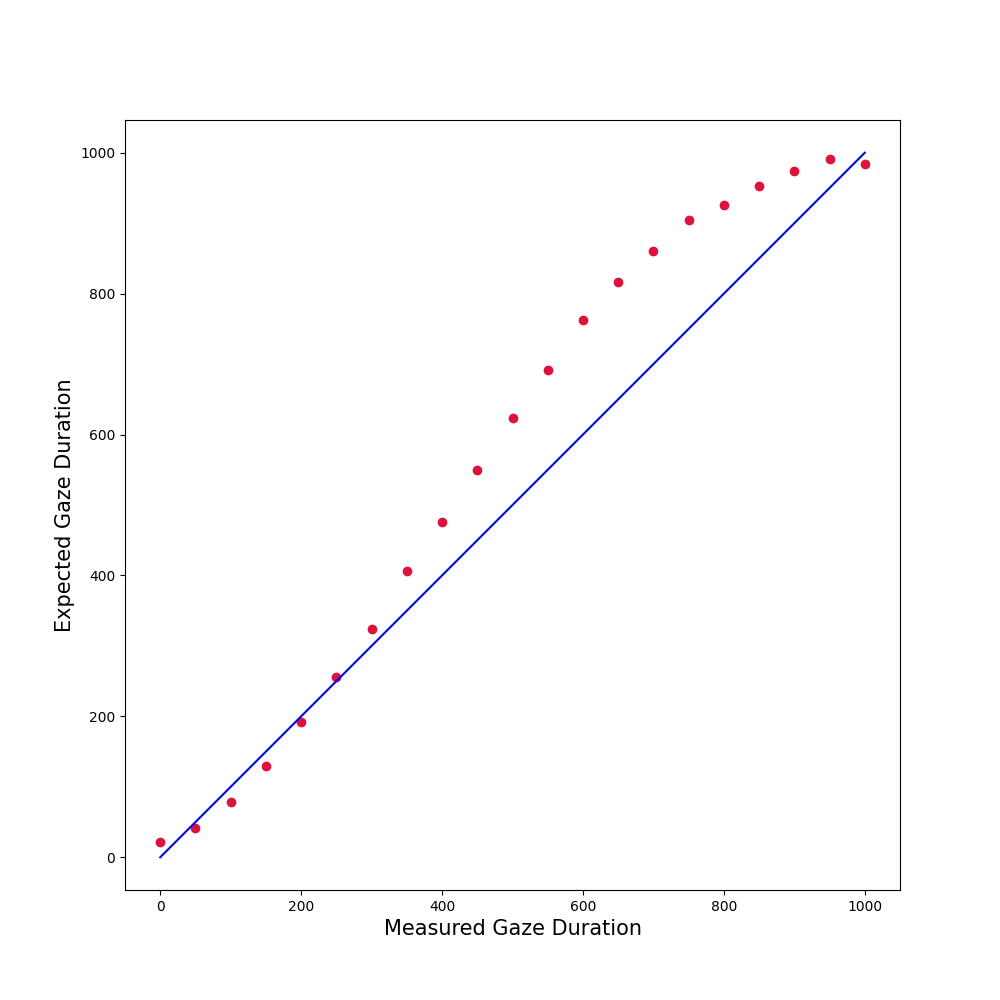
\includegraphics[scale=0.5]{../results/Measured_vs_expected.png}
\caption{Measured Gaze Duration Versus Expected Gaze Duration. \\\hspace{\textwidth} 
MREC ad appearing on screen for 1s with 70px Mean Error in Fixation}
\label{fig:measured_vs_expected}
\end{figure}

The result shown in Figure \ref{fig:measured_vs_expected} is indicative of what we 
see under multiple variations of the simulation configuration. 
At lower meaurement values there is a tendency for the measurement to be an 
accurate estimation of true gaze duration, while 
at higher values it tends toward an under-estimation of the true gaze duration.
This problem is worse for the model with the biased error, but it is mitigated
when the biased error comes from a model with higher precision. This is potentially
due to the fact that the high prescion scenario has lower tendency for gaze to be 
pushed off screen.  

We next examined the way that exected error in the gaze duration estimate tracks with 
expected error in the gaze fixation points. This involved calculating the mean absolute
error in gaze duration for each of the mean fixation error validation files. 
We performed this calculation using two methods. The first method, labelled uniform, 
assumes that all measured values are equally likely. The second method, labelled exponential,
assumes that low measurements are much more likely than higher measurement, and that 
this drop in likelihood follows an approximately exponential distribution.

\begin{figure}[h!]
\centering
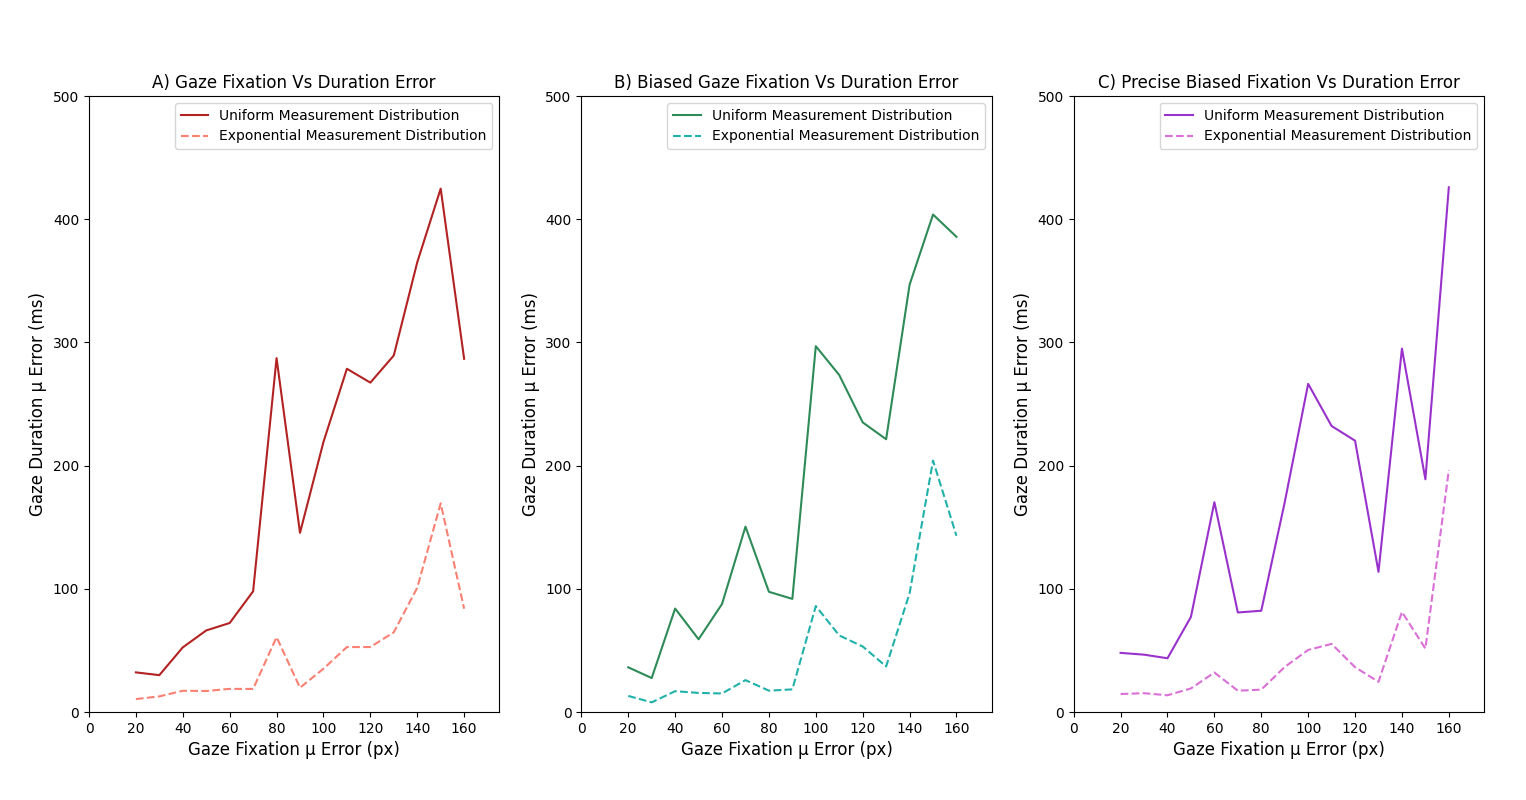
\includegraphics[scale=0.4]{../results/Fixation_vs_duration_error.png}
\caption{Fixation error versus gaze duration error.}
\label{fig:fixation_vs_duration}
\end{figure}

As shown in Figure \ref{fig:fixation_vs_duration} we see that the error in gaze duration
grows with error in fixation points, as would be expected. However, when we use the 
exponential weighting to calculate the expected error in duration the gaze duration 
error grows much slower than in the uniform case. This suggests that the observed 
tendency toward smaller measurements in advertising area of interest studies means 
lower expected error overall. This pattern is true for the centrally distributed 
error (A) as well as the biased calibration error (B) and precise biased calibration
error (C) scenarios.

In addition, the additional error in gaze duration we see when the error is biased
in a particular direction (shown in B) is partly mitigated by a fixation model that
is more precise (shown in C). This suggests that a precise fixation sampling process
is able to partly overcome the false positive and false negatives of an error prone gaze
fixation model.

In our final experiment we look at the effect of both the size of the measured 
gaze duration and the mean error of fixation on the expected error in gaze duration.
We conduct this experiment using only the unbiased synthetic data in order to understand
how error centred on true fixation points relates to error in gaze duration across the
range of measurement. We display these results as a three dimensional expected error 
surface over these two key dimensions in Figure \ref{fig:error_surface}

\begin{figure}[h!]
\centering
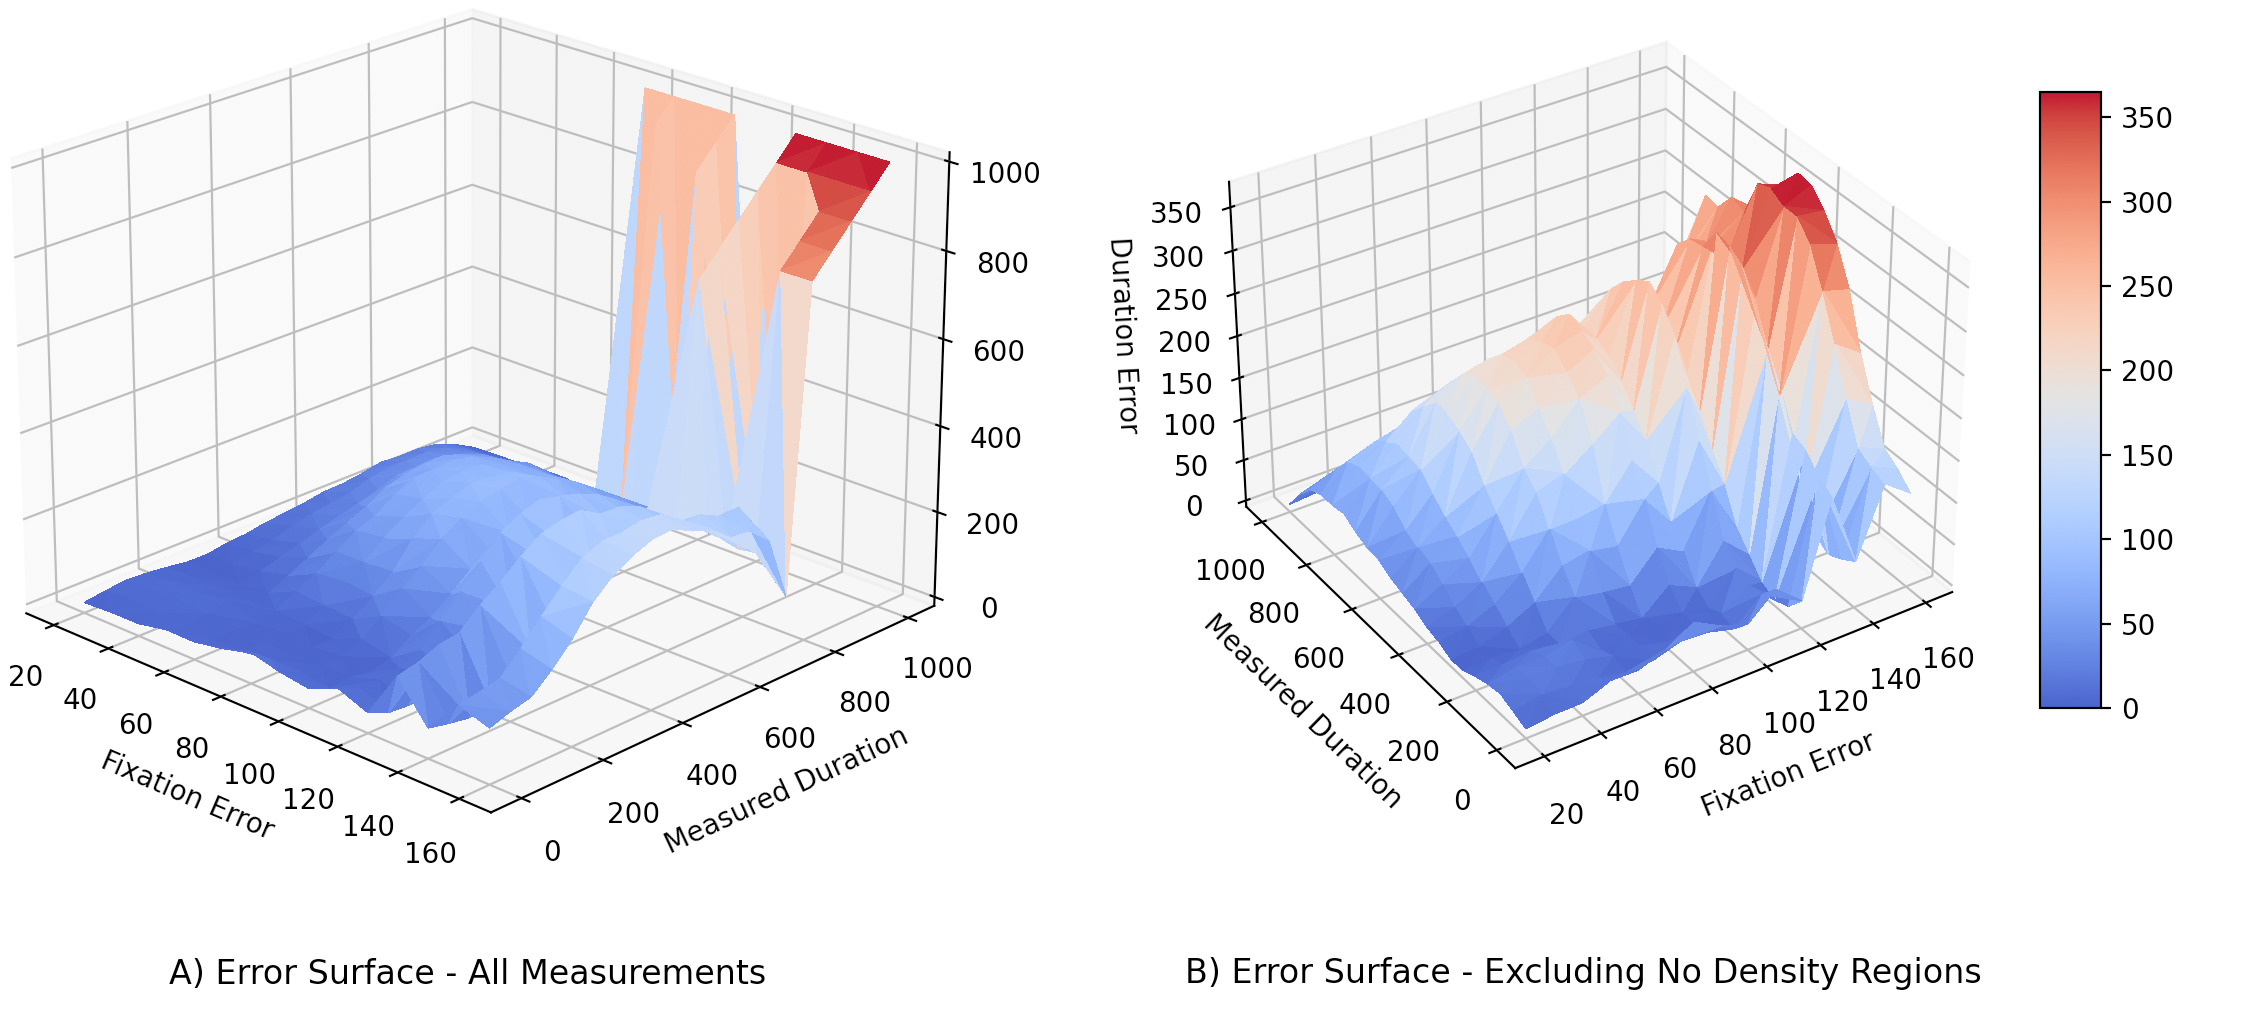
\includegraphics[scale=0.4]{../results/Error_surface.png}
\caption{Mean gaze duration error over measured error and fixation MAE.}
\label{fig:error_surface}
\end{figure}

The left hand plot shows the complete error surface in which you will observe large 
spikes in
error in the corner corresponding to both high mean error for the fixation models and 
high measurements of gaze duration. 
This effect is caused by a complete absence of probability density in these
regions, meaning that the error is maximal because the expected value is zero. This effect 
was consistently observed for 
eye tracking models with high mean fixation error and when the measured duration was high. 
The consequence of this is that our model estimates that when fixation error is this high, 
measurements of these values
become extremely unlikley to be observed.

We added the right hand plot in Figure \ref{fig:error_surface} to illustrate the error surface
in the absence of these deceptive outliers. We see that, in general, the expected error in a gaze
duration measurement is maximal around the mid point of the measurement range. The effect is lessened by 
lower mean error in the fixation models, but remains consistent for all levels of fixation error.

\section{Conclusion}

We have demonstrated that the statistial information contained in eye tracking calibration
data can be utilised for estimating errors in gaze duration estimation. The process involves
simulating the distribution of measured duration for each possible true duration, 
and then inverting it with Bayes rule into a distribution over true duration for a 
given measurement.

We have released this approach as the open source application \textit{gazerr} and 
used it to explore the relationship between fixation error and duration error, under
range of realistic error profiles when looking at measuring attention on a standard
size ad within a mobile screen. Our results show that the nature
of the error in gaze duration tends to depend on the size of the measurement. 
Smaller measurements tend to have lower expected error while larger measurements 
tend toward under prediction. 
We plotted the relationship between expected error and saw that the observed 
tendency toward smaller duration measurements 
(estimated with an psuedo-exponential distribution) delivers a slower growing
expected duration error with the mean error in fixation points.

Finally, our simulations revealed that for large error in fixation points, 
certain measurements become so unlikely that our Monte Carlo simulations placed 
none of the probability density in those regions. 
This strongly suggests that an additional downside to large fixation point error
is a reduced range of measurement for area of interest studies.

\bibliographystyle{IEEEtran}
\bibliography{refs}

\end{document}
